\newcommand{\casebox}[2]{\par\noindent{\setlength{\fboxsep}{1pt}\colorbox{#1}{\parbox{\dimexpr\linewidth-2\fboxsep\relax}{\raggedright\fontsize{6}{6.5}\selectfont #2}}}\par}
\section{Proof of Proposition 1}
\label{app:proof}
\textbf{Proposition 1.} \textit{With equal format scores, $R_{\mathrm{P}}$ is maximal only where the learning signal peaks and minimal where it vanishes.}\vspace{-2mm}
\begin{proof}
Let $q$ be a valid question with Solver trajectories $\{\rho^{j}\}_{j=1}^{n}$, answer scores $s_j\in[0,1]$ and mean $\bar{s}$ as in Equation~\ref{eq:cbar}, and format scores that all equal $f$. Then $R_{\mathrm{S}}(\rho^{j})=\lambda_{\mathrm{fmt}}f+\lambda_{\mathrm{ans}}s_j$ is a positive affine map of $s_j$, and since the group-normalized advantage is invariant to such maps, $\hat{A}^{j}=(s_j-\bar{s})/\sigma$ with $\sigma=\sqrt{\sigma^{2}(q)}$ when $\sigma>0$, and $\hat{A}^{j}=0$ when $\sigma=0$.

\emph{Learning signal.} We measure the Solver's learning signal on $q$ by the mean absolute advantage of its group,
\begin{equation}
\label{eq:signal}
S(q)=\frac1n\sum_{j=1}^{n}\bigl|\hat{A}^{j}\bigr|.
\end{equation}
If $\sigma^{2}(q)=0$, all scores are equal, every $\hat{A}^{j}=0$, and $S(q)=0$. Otherwise the normalized advantages satisfy $\frac1n\sum_{j}(\hat{A}^{j})^{2}=1$, so by the Cauchy--Schwarz inequality $S(q)\le1$, with equality if and only if all $|\hat{A}^{j}|$ are equal, i.e., half of the scores lie at $\bar{s}+\sigma$ and the other half at $\bar{s}-\sigma$.

\emph{Maximum and minimum.} Since $0\le s_j\le1$, we have $s_j^{2}\le s_j$ and hence $\sigma^{2}(q)=\frac1n\sum_{j}s_j^{2}-\bar{s}^{2}\le\bar{s}(1-\bar{s})\le\tfrac14$, where the first inequality is tight only if every $s_j\in\{0,1\}$ and the second only if $\bar{s}=\tfrac12$. Hence $R_{\mathrm{P}}(q)$ reaches its maximum $1$ only when half of the trajectories score $1$ and the other half score $0$; there $\hat{A}^{j}=\pm1$ and $S(q)=1$, its largest possible value. Conversely, $R_{\mathrm{P}}(q)$ takes its minimum $\exp(-\tfrac{1}{32h})$ exactly when $\sigma^{2}(q)=0$, which is exactly when $S(q)=0$. With $n=5$, an even split is impossible and $\sigma^{2}(q)\le0.24$, attained only by a $2{:}3$ split between scores $0$ and $1$.
\end{proof}

\textbf{Remark.} The adversarial and triangular rewards of Section~\ref{sec:ablation} are functions of the success rate $\bar{c}$. The adversarial reward peaks at $\bar{c}=0$, where every trajectory misses, all scores are $0$, and $S(q)=0$. The triangular reward peaks at $\bar{c}=\tfrac12$ but, like the adversarial reward, does not reflect how much of the answer set each trajectory recovers.

\section{Algorithm Details}
\label{app:algorithm}
\begin{table*}[t]
\centering
\begin{minipage}[t]{0.485\textwidth}
\caption{\textbf{Proposer on a $2i$ task.} It explores both anchors and asks for the country they share.}\label{tab:case-pair-proposer}
\casebox{gray!20}{\textbf{Role:} Proposer \quad \textbf{Task:} Jèrriais $\leftarrow$ location.\allowbreak{}country.\allowbreak{}languages\_\allowbreak{}spoken-- Ans@ ; French --language.\allowbreak{}human\_\allowbreak{}language.\allowbreak{}countries\_\allowbreak{}spoken\_\allowbreak{}in $\rightarrow$ Ans@ \quad \textbf{Executed answer:} Jersey}
\casebox{blue!10}{\texttt{<think>} The Path suggests that Jèrriais is a language spoken in a country, and French is also spoken in that same country. The question should ask for the country where both Jèrriais and French are spoken. Let's explore the knowledge graph to identify the country. \texttt{</think>}}
\casebox{green!10}{\texttt{<kg-query>} get\_\allowbreak{}relations("Jèrriais") \texttt{</kg-query>}}
\casebox{yellow!10}{\texttt{<information>} location.\allowbreak{}country.\allowbreak{}languages\_\allowbreak{}spoken, language.\allowbreak{}human\_\allowbreak{}language.\allowbreak{}main\_\allowbreak{}country, language.\allowbreak{}human\_\allowbreak{}language.\allowbreak{}language\_\allowbreak{}family, language.\allowbreak{}language\_\allowbreak{}family.\allowbreak{}languages, people.\allowbreak{}ethnicity.\allowbreak{}languages\_\allowbreak{}spoken, language.\allowbreak{}human\_\allowbreak{}language.\allowbreak{}countries\_\allowbreak{}spoken\_\allowbreak{}in \texttt{</information>}}
\casebox{blue!10}{\texttt{<think>} The relation 'location.\allowbreak{}country.\allowbreak{}languages\_\allowbreak{}spoken' confirms that Jèrriais is spoken in a country. Let's use 'get\_\allowbreak{}triples' to find out which country it is. \texttt{</think>}}
\casebox{green!10}{\texttt{<kg-query>} get\_\allowbreak{}triples("Jèrriais", ["location.\allowbreak{}country.\allowbreak{}languages\_\allowbreak{}spoken"]) \texttt{</kg-query>}}
\casebox{yellow!10}{\texttt{<information>} [Jersey, location.\allowbreak{}country.\allowbreak{}languages\_\allowbreak{}spoken, Jèrriais] \texttt{</information>}}
\casebox{blue!10}{\texttt{<think>} We have determined that Jèrriais is spoken in Jersey. Now, we need to find out if French is also spoken in Jersey. Let's check the languages spoken in Jersey using the relation 'language.\allowbreak{}human\_\allowbreak{}language.\allowbreak{}countries\_\allowbreak{}spoken\_\allowbreak{}in'. \texttt{</think>}}
\casebox{green!10}{\texttt{<kg-query>} get\_\allowbreak{}triples("Jersey", ["language.\allowbreak{}human\_\allowbreak{}language.\allowbreak{}countries\_\allowbreak{}spoken\_\allowbreak{}in"]) \texttt{</kg-query>}}
\casebox{yellow!10}{\texttt{<information>} [French, language.\allowbreak{}human\_\allowbreak{}language.\allowbreak{}countries\_\allowbreak{}spoken\_\allowbreak{}in, Jersey], [English Language, language.\allowbreak{}human\_\allowbreak{}language.\allowbreak{}countries\_\allowbreak{}spoken\_\allowbreak{}in, Jersey], [Jèrriais, language.\allowbreak{}human\_\allowbreak{}language.\allowbreak{}countries\_\allowbreak{}spoken\_\allowbreak{}in, Jersey] \texttt{</information>}}
\casebox{blue!10}{\texttt{<think>} The information confirms that French is indeed spoken in Jersey. Thus, the answer to the question is Jersey. \texttt{</think>}}
\casebox{lightblue}{\texttt{<result>} \{"question": "In which country are both Jèrriais and French spoken?"\} \texttt{</result>}}
\end{minipage}\hfill
\begin{minipage}[t]{0.485\textwidth}
\caption{\textbf{Solver on the question of Table~\ref{tab:case-pair-proposer}.} It intersects the countries of the two languages.}\label{tab:case-pair-solver}
\casebox{gray!20}{\textbf{Role:} Solver \quad \textbf{Question:} In which country are both Jèrriais and French spoken?}
\casebox{blue!10}{\texttt{<think>} 1. The initial entities are Jèrriais and French. I need to find the country where both Jèrriais and French are spoken. I will start by querying the knowledge graph to find related information about Jèrriais and its spoken locations. \texttt{</think>}}
\casebox{green!10}{\texttt{<kg-query>} get\_\allowbreak{}relations("Jèrriais") \texttt{</kg-query>}}
\casebox{yellow!10}{\texttt{<information>} location.\allowbreak{}country.\allowbreak{}languages\_\allowbreak{}spoken, language.\allowbreak{}human\_\allowbreak{}language.\allowbreak{}main\_\allowbreak{}country, language.\allowbreak{}human\_\allowbreak{}language.\allowbreak{}language\_\allowbreak{}family, language.\allowbreak{}language\_\allowbreak{}family.\allowbreak{}languages, people.\allowbreak{}ethnicity.\allowbreak{}languages\_\allowbreak{}spoken, language.\allowbreak{}human\_\allowbreak{}language.\allowbreak{}countries\_\allowbreak{}spoken\_\allowbreak{}in \texttt{</information>}}
\casebox{blue!10}{\texttt{<think>} I now have some potential relations to explore. I will query the knowledge graph with the first relation "location.\allowbreak{}country.\allowbreak{}languages\_\allowbreak{}spoken" to see if it can provide the country where both languages are spoken. \texttt{</think>}}
\casebox{green!10}{\texttt{<kg-query>} get\_\allowbreak{}triples("Jèrriais", ["location.\allowbreak{}country.\allowbreak{}languages\_\allowbreak{}spoken"]) \texttt{</kg-query>}}
\casebox{yellow!10}{\texttt{<information>} [Jersey, location.\allowbreak{}country.\allowbreak{}languages\_\allowbreak{}spoken, Jèrriais] \texttt{</information>}}
\casebox{blue!10}{\texttt{<think>} The knowledge graph has shown that Jèrriais is spoken in Jersey. Now, to find out if French is also spoken there, I will query the knowledge graph with the relation "language.\allowbreak{}human\_\allowbreak{}language.\allowbreak{}countries\_\allowbreak{}spoken\_\allowbreak{}in" to verify if French is spoken in Jersey. \texttt{</think>}}
\casebox{green!10}{\texttt{<kg-query>} get\_\allowbreak{}triples("French", ["language.\allowbreak{}human\_\allowbreak{}language.\allowbreak{}countries\_\allowbreak{}spoken\_\allowbreak{}in"]) \texttt{</kg-query>}}
\casebox{yellow!10}{\texttt{<information>} [French, language.\allowbreak{}human\_\allowbreak{}language.\allowbreak{}countries\_\allowbreak{}spoken\_\allowbreak{}in, Dominica], [French, language.\allowbreak{}human\_\allowbreak{}language.\allowbreak{}countries\_\allowbreak{}spoken\_\allowbreak{}in, Mali], [French, language.\allowbreak{}human\_\allowbreak{}language.\allowbreak{}countries\_\allowbreak{}spoken\_\allowbreak{}in, Chad], [French, language.\allowbreak{}human\_\allowbreak{}language.\allowbreak{}countries\_\allowbreak{}spoken\_\allowbreak{}in, Jersey], [French, language.\allowbreak{}human\_\allowbreak{}language.\allowbreak{}countries\_\allowbreak{}spoken\_\allowbreak{}in, Ivory Coast] \texttt{</information>}}
\casebox{blue!10}{\texttt{<think>} I have confirmed that French is spoken in Jersey alongside Jèrriais. Therefore, the country where both languages are spoken is Jersey. \texttt{</think>}}
\casebox{lightblue}{\texttt{<answer>} ["Jersey"] \texttt{</answer>}}
\end{minipage}
\end{table*}


\begin{figure}[t]
\centering
\begin{minipage}[t]{\linewidth}
\makeatletter\@twocolumnfalse\makeatother %
\begin{algorithm}[H]
\SetAlgoLined
\DontPrintSemicolon
\KwIn{KG $\mathcal{G}$; pattern set $\mathcal{P}$; seed pool $\mathcal{E}_{\mathrm{seed}}$; per-pattern target $N$; attempt budget $T$; answer cap $\kappa$}
\KwOut{task set $\mathcal{D}_{\mathrm{SVTS}}$}
$\mathcal{D}\leftarrow\varnothing$\;
\ForEach{$pat\in\mathcal{P}$}{
  $n\leftarrow 0$;\quad $t\leftarrow 0$\;
  \While{$n<N$ \textbf{and} $t<T$}{
    $t\leftarrow t+1$;\quad sample seed $s\in\mathcal{E}_{\mathrm{seed}}$\;
    $\pi\leftarrow$ random walk realizing $pat$ from $s$ in $\mathcal{G}$\;
    \lIf{$\pi=\bot$}{\textbf{continue}}
    $G_Q\leftarrow\mathrm{assemble}(pat,\pi)$;\quad $Q\leftarrow\mathrm{Compile}(G_Q)$\;
    $\mathcal{A}_Q\leftarrow\mathrm{Execute}(Q,\mathcal{G})$\;
    \lIf{$\mathcal{A}_Q=\varnothing$ \textbf{or} $|\mathcal{A}_Q|\ge\kappa$ \textbf{or} $\neg\mathrm{Named}(\mathcal{A}_Q)$}{\textbf{continue}}
    $\mathcal{D}\leftarrow\mathcal{D}\cup\{(G_Q,\mathcal{E}_Q,\mathcal{A}_Q)\}$;\quad $n\leftarrow n+1$\;
  }
}
\Return{$\mathcal{D}_{\mathrm{SVTS}}\leftarrow\mathcal{D}$}\;
\caption{Symbolically Verifiable Topology Synthesis}
\label{alg:svts}
\end{algorithm}
\end{minipage}
\vspace{-2mm}
\end{figure}

\paragraph{SVTS}
As shown in Table~\ref{tab:patterns} and Algorithm~\ref{alg:svts}, SVTS repeats grounding, compilation, and execution for each of the six query patterns until it collects $N$ tasks or exhausts $T$ attempts. Grounding walks from a seed entity to bind the variables and relations of the pattern to real facts; the resulting query graph is compiled into an executable query and evaluated on the graph, and queries with empty, at least $\kappa$, or unnameable answers are discarded before training.

\begin{table}[!h]
\caption{\textbf{Basic logic query patterns.} $v_a$: anchor entity; $x$: answer variable; $y_i$: intermediate variables; $r_i$: relations.}
\label{tab:patterns}
\centering
\footnotesize
\setlength{\tabcolsep}{5pt}
\renewcommand{\arraystretch}{1.1}
\newcommand{\patternimg}[1]{%
  \raisebox{-0.5\height}{\includegraphics[scale=0.9]{#1}}%
}

\resizebox{\columnwidth}{!}{%
\begin{tabular}{c c l}
\toprule
\textbf{Pattern} & \textbf{Structure}
& \textbf{Logical query} \\
\midrule

$1p$ &
\patternimg{figures/1P.pdf} &
$\phi(x)=r_1(v_a,x)$ \\[2pt]

$2p$ &
\patternimg{figures/2P.pdf} &
$\phi(x)=\exists y:\ r_1(v_a,y)\wedge r_2(y,x)$ \\[2pt]

$3p$ &
\patternimg{figures/3P.pdf} &
$\phi(x)=\exists y_1,y_2:\ r_1(v_a,y_1)\wedge r_2(y_1,y_2)
\wedge r_3(y_2,x)$ \\[2pt]

$2i$ &
\patternimg{figures/2i.pdf} &
$\phi(x)=r_1(v_{a_1},x)\wedge r_2(v_{a_2},x)$ \\[2pt]

$ip$ &
\patternimg{figures/IP.pdf} &
$\phi(x)=\exists y:\ r_1(v_{a_1},y)\wedge r_2(v_{a_2},y)
\wedge r_3(y,x)$ \\[2pt]

$pi$ &
\patternimg{figures/PI.pdf} &
$\phi(x)=\exists y:\ r_1(v_{a_1},y)\wedge r_2(y,x)
\wedge r_3(v_{a_2},x)$ \\[2pt]

\bottomrule
\end{tabular}%
}
\end{table}

\section{Experimental Details}
\label{app:experimental-details}
\begin{figure}[t]
\centering
\begin{minipage}{0.32\linewidth}
  \centering
  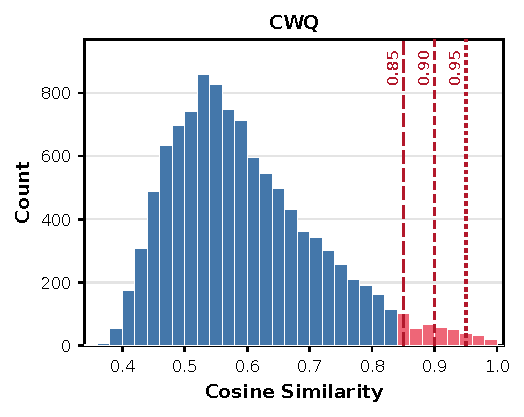
\includegraphics[width=\linewidth]{figures/A_2_similarity_cwq.pdf}\\[-0.2em]
  {\scriptsize (a) CWQ}
\end{minipage}\hfill
\begin{minipage}{0.32\linewidth}
  \centering
  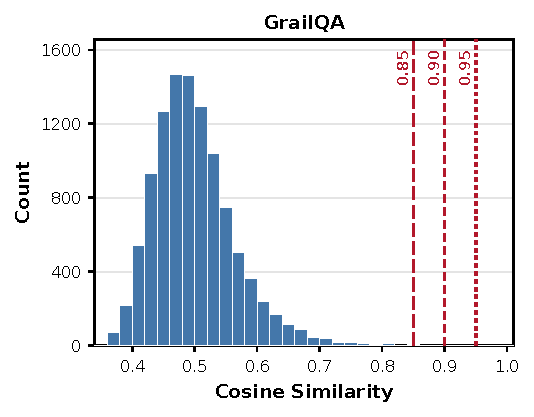
\includegraphics[width=\linewidth]{figures/A_2_similarity_grailqa.pdf}\\[-0.2em]
  {\scriptsize (b) GrailQA}
\end{minipage}\hfill
\begin{minipage}{0.32\linewidth}
  \centering
  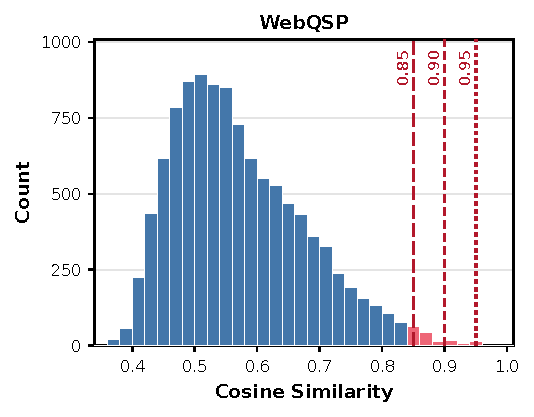
\includegraphics[width=\linewidth]{figures/A_2_similarity_webqsp.pdf}\\[-0.2em]
  {\scriptsize (c) WebQSP}
\end{minipage}
\caption{\textbf{Semantic contamination analysis.} Max cosine similarity of synthesized questions to each test set.}
\label{fig:contamination}
\end{figure}
\begin{table}[t]
\caption{\textbf{Settings of EoG.} Hyperparameters of self-play training with Qwen-2.5-7B-Instruct on Freebase.}
\label{tab:hyperparams}
\centering
\small
\setlength{\tabcolsep}{4pt}
\renewcommand{\arraystretch}{1.0}
\begin{tabular}{lc}
\toprule
\textbf{Parameter} & \textbf{Value} \\
\midrule
Training data & SVTS tasks \\
Training steps & 140 \\
Train / PPO mini-batch size & 256 / 128 \\
Actor learning rate & $1\times10^{-6}$ \\
KL loss coefficient & 0.01 \\
Rollout samples ($n$) & 5 \\
Max response length & 2560 \\
Max assistant turns & 15 \\
Rollout temperature & 0.8 \\
Solver / Proposer estimator & GRPO / REINFORCE \\
Solver reward & $0.8\,\mathrm{F1}+0.2\,R_{\mathrm{fmt}}$ \\
\bottomrule
\end{tabular}
\end{table}

\subsection{Datasets}
\label{app:datasets}
On Freebase, \textbf{WebQSP}~\citep{webqsp} contains single-hop and two-hop questions, \textbf{CWQ}~\citep{cwq} extends WebQuestions with multi-entity constraints, conjunctions, and superlatives, and \textbf{GrailQA}~\citep{grailqa} tests i.i.d., compositional, and zero-shot generalization. On Wikidata, \textbf{GTSQA}~\citep{GTSQA} provides $1{,}622$ test questions with gold answer subgraphs, and \textbf{WikiWebQuestions}~\citep{wikiwebquestions} migrates WebQuestions to Wikidata with re-annotated SPARQL queries. \textbf{IndustryCarBench} is a domain benchmark that we build on a real-world automotive-aesthetics KG covering car models, design elements, attributes, colors, materials, and brands; it contains $500$ test questions written by domain experts, with gold answers executable on the graph and has no annotated training set. EoG never uses the annotated training questions of any benchmark; only KG-R1$^\dagger$ does.

\subsection{Baselines and Metrics}
\label{app:baselines}
\label{app:metrics}
All baselines use the same backbone as the compared EoG model. IO answers directly, CoT~\citep{CoT} reasons step by step, and SC~\citep{Self-Consistency} takes a majority vote over sampled CoT chains. ReAct~\citep{React} interleaves thoughts, graph-tool calls, and observations with the tools and Solver prompt of EoG. ToG~\citep{ToG} runs LLM-guided beam search over entities and relations, PoG~\citep{PoG} decomposes a question into subgoals with adaptive exploration and self-correction, and CoR~\citep{CoR} builds a relation chain and filters the reachable candidates with the question constraints. Text-Based Retrieval selects the top-$k$ verbalized triples by embedding similarity, and Graph Reranker reranks the triples within the $L$-hop neighborhood of the anchors. Following~\citep{ToG,PoG}, Hit@1 checks whether the normalized prediction exactly matches any gold answer, and F1 measures the overlap between the predicted and gold answer lists of each question.

\subsection{Implementation Details}
\label{app:training}

We train EoG with Verl on 8 GH200 GPUs across two nodes, using FSDP with CPU offloading of parameters and optimizer states and SGLang for multi-turn rollouts; Table~\ref{tab:hyperparams} lists the hyperparameters. KG-R1$^\dagger$ converts the official training splits of WebQSP, CWQ, and GrailQA into the Solver format, which yields $3{,}058$, $27{,}623$, and $36{,}954$ questions, and trains one model per dataset. It uses the same backbone, Solver prompt, graph tools, and Freebase endpoint as EoG, so only the source of the training questions differs. Its reward is the F1 of EoG without the format term.

\subsection{Synthetic Data Analysis}
\label{app:contamination}

\paragraph{Topology coverage.}
Synthesized questions on Freebase cover all six patterns: the chain patterns $1p$ ($22.4\%$), $2p$ ($20.6\%$), and $3p$ ($16.5\%$), and the intersection patterns $2i$ ($17.7\%$), $pi$ ($9.5\%$), and $ip$ ($13.3\%$). The Solver must learn path expansion, constraint intersection, and intermediate-variable tracking rather than fit a single pattern.

\paragraph{Domain coverage.}
The questions cover 20 domains, including Places \& Geography ($14.2\%$), Film \& Television ($13.2\%$), Government, Law \& Military ($12.6\%$), People \& Society ($8.7\%$), and Sports ($8.4\%$); the top three together account for only $40.0\%$. Training signals are therefore not confined to a few dense subgraphs of Freebase.

\paragraph{Test-set leakage.}
To rule out test-set leakage, we encode each question with BGE-M3 and take the maximum cosine similarity between each synthetic question and the questions of each Freebase test set (Figure~\ref{fig:contamination}). Only $4.57\%$, $2.28\%$, and $0.71\%$ of the synthetic questions exceed $0.85$, $0.90$, and $0.95$, respectively, and the mean similarity is $0.634$, so there is no meaningful leakage between the synthetic training data and the Freebase evaluation sets.

\section{Case Study}
\label{app:case-study}
Tables~\ref{tab:case-pair-proposer} and~\ref{tab:case-pair-solver} give the full trajectories of the case in Section~\ref{sec:case-study}. The Proposer starts from Jèrriais, finds that it is spoken in Jersey, and queries the languages of Jersey to confirm that French is spoken there before asking. The Solver instead retrieves every country where French is spoken, among them Mali, Chad, and Jersey, and keeps the one shared with Jèrriais, the executed answer.

